% !TeX program = xelatex
\documentclass[12pt,a4paper]{ctexart}
\usepackage{geometry}
\geometry{left=2.5cm,right=2.5cm,top=2.5cm,bottom=2.5cm}
\usepackage{fancyhdr}
\usepackage{graphicx}
\usepackage{amsmath}
\usepackage{float}
\usepackage{caption}
\captionsetup{font=small,labelfont=bf}
\usepackage[hidelinks]{hyperref}
\usepackage{listings}
\usepackage{xcolor}
\usepackage{booktabs}

% ---------- 代码块样式（与第二周一致） ----------
\lstset{
    basicstyle=\ttfamily\small,
    keywordstyle=\color{blue},
    commentstyle=\color{gray},
    stringstyle=\color{red},
    showstringspaces=false,
    breaklines=true,
    frame=single,
    backgroundcolor=\color{gray!10},
    numbers=left,
    numberstyle=\tiny\color{gray},
    tabsize=4,
    xleftmargin=2em,
    xrightmargin=2em,
}

% ---------- 中文字体 ----------
\setCJKmainfont{Noto Serif CJK SC}
\setCJKsansfont{Noto Sans CJK SC}
\setCJKmonofont{Noto Sans Mono CJK SC}

% ---------- 页眉页脚 ----------
\pagestyle{fancy}
\fancyhf{}
\fancyhead[C]{\small 系统开发工具基础 · 实验报告（第一周）}
\fancyfoot[C]{\thepage}
\renewcommand{\headrulewidth}{0.4pt}
\renewcommand{\footrulewidth}{0pt}

% ---------- 标题格式 ----------
\usepackage{titlesec}
\titleformat{\section}{\Large\bfseries\centering}{第\thesection 题}{1em}{}
\titleformat{\subsection}{\normalsize\bfseries}{\arabic{subsection}}{1em}{}
\renewcommand{\baselinestretch}{1.3}

\begin{document}

% ==================== 封面 ====================
\begin{center}
    {\Huge\bfseries 系统开发工具基础} \\[0.5cm]
    {\LARGE 每周课上实验报告} \\[0.8cm]
    {\large 第一周（2026年8月24日）} \\[2cm]
    \large
    \begin{tabular}{rl}
        姓\qquad 名： & 李永铖 \\
        学\qquad 号： & 25030021039 \\
        实验日期： & 2026年8月24日
    \end{tabular} \\[2cm]
    \today
\end{center}
\newpage

% ==================== 实验概述与环境 ====================
\section*{实验概述}
\addcontentsline{toc}{section}{实验概述}

本次实验为第一周的四道课上练习题，涵盖 Shell 基础与文件系统、Shell 文本处理、Git 版本控制以及 LaTeX 文档编辑。通过动手实践，巩固了命令行操作、管道与过滤、分支合并冲突解决以及技术文档的编写与编译能力。

\subsection*{实验环境}
\begin{itemize}
    \item 操作系统：Windows 11 + WSL2 (Debian)
    \item Shell：bash 5.0
    \item Git：1.9.1（初始未安装，后自行安装）
    \item LaTeX 引擎：XeLaTeX（通过 latexmk 调用）
    \item 中文宏包：xeCJK（需安装 texlive-lang-chinese）
    \item 中文字体：Noto Serif CJK SC / Noto Sans CJK SC
\end{itemize}

\subsection*{遇到的问题与解决}
\begin{enumerate}
    \item \textbf{Git 未安装}：使用 \texttt{sudo apt install git} 安装。
    \item \textbf{latexmk 默认调用 pdflatex}：通过 \texttt{latexmk -xelatex} 指定引擎。
    \item \textbf{xeCJK.sty 缺失}：安装 \texttt{texlive-lang-chinese} 并执行 \texttt{sudo texhash}。
    \item \textbf{中文字体未配置}：安装 \texttt{fonts-noto-cjk} 并用 \verb|\setCJKmainfont| 指定。
    \item \textbf{编译器必须为 XeLaTeX}：否则 Unicode 字符报错。
\end{enumerate}

\newpage

% ==================== 第1题 ====================
\section{含空格文件名的批量整理}

\subsection{操作步骤}
\begin{enumerate}
    \item 创建目录 \texttt{q01} 及其子目录 \texttt{input/docs}、\texttt{input/tmp}。
    \item 使用 \texttt{echo -e} 创建含多行内容的文件，并用 \texttt{touch} 创建空文件。
    \item 显示绝对路径，用 \texttt{ls -la} 列出 \texttt{input} 下所有项目。
    \item 使用 \texttt{find ... -exec cp --parents} 复制所有 \texttt{.txt} 文件到 \texttt{work/<学号>}，保留目录结构。
    \item 修改权限：目录 750，文件 640。
    \item 用 \texttt{find -printf} 生成 \texttt{inventory.txt}，包含相对路径和字节数。
\end{enumerate}

\subsection{核心命令}
\begin{lstlisting}[language=bash]
# 创建目录与文件
mkdir -p input/docs input/tmp
echo -e "alpha\nbeta" > input/docs/notesone.txt
touch input/tmp/empty.txt

# 复制并保留结构
find input -name "*.txt" -exec cp --parents {} work/20240101/ \;
# 权限设置
find work/20240101 -type d -exec chmod 750 {} \;
find work/20240101 -type f -exec chmod 640 {} \;

# 生成清单
find work/20240101 -type f -printf "%P %s\n" > inventory.txt
\end{lstlisting}

\subsection{结果验证}
执行 \texttt{ls -lR work/20240101} 查看文件结构；\texttt{cat inventory.txt} 显示如下：
\begin{lstlisting}
input/docs/notesone.txt 12
input/docs/secret.txt 7
input/tmp/empty.txt 0
\end{lstlisting}
权限与要求一致。
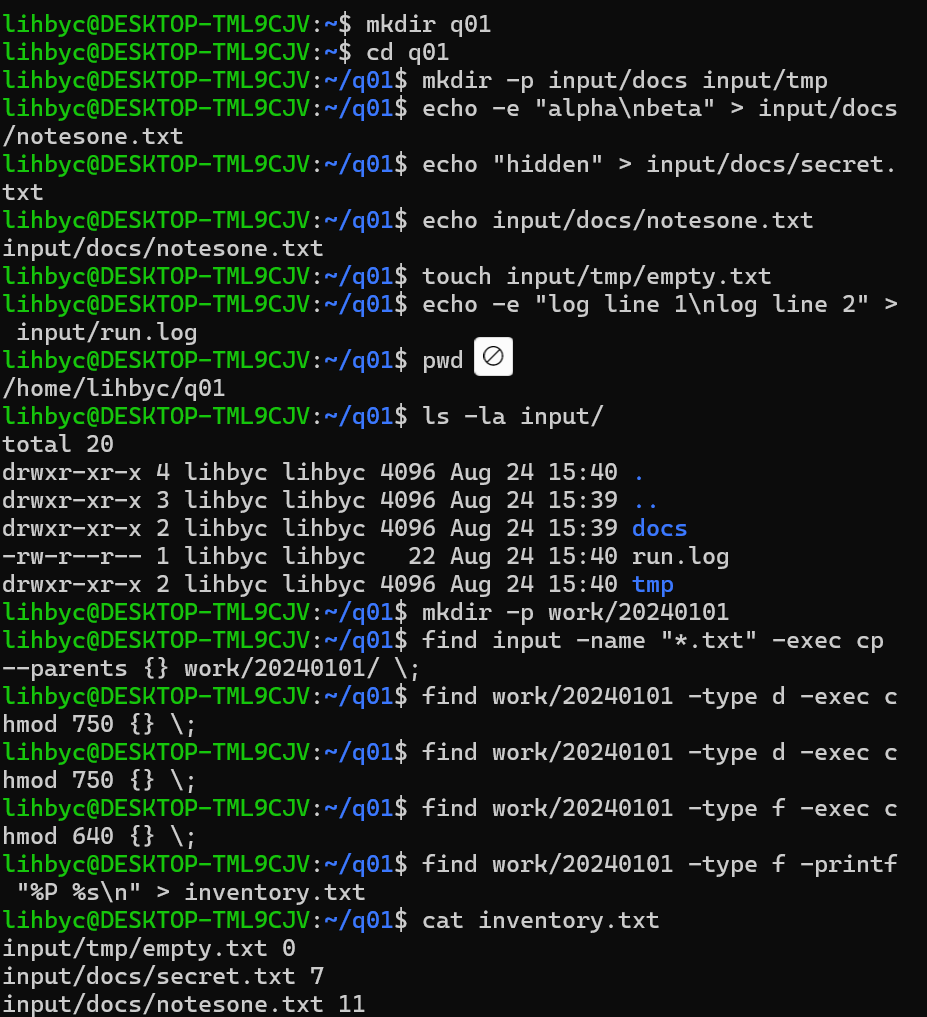
\includegraphics[width=0.6\textwidth]{q01.png}

\newpage

% ==================== 第2题 ====================
\section{随机访问日志统计}

\subsection{操作步骤}
\begin{enumerate}
    \item 创建 \texttt{q02} 目录，写入 \texttt{access.csv} 数据。
    \item 编写 \texttt{analyze.sh} 脚本，包含参数检查和错误处理。
    \item 使用 \texttt{awk} 统计 5xx 状态码的路径次数，并用 \texttt{sort}、\texttt{head} 输出前两名。
    \item 使用第二个 \texttt{awk} 计算平均延迟，保留两位小数。
    \item 分别对正常文件和不存在文件运行脚本，验证错误处理。
\end{enumerate}

\subsection{核心代码}
\begin{lstlisting}[language=bash]
#!/bin/bash
if [ $# -ne 1 ]; then
    echo "Usage: $0 <csv_file>" >&2; exit 1
fi
if [ ! -f "$1" ]; then
    echo "Error: File '$1' not found" >&2; exit 1
fi

# 5xx 路径统计
awk -F',' 'NR>1 && ($4>=500 && $4<600) {count[$3]++} END {for(p in count) print count[p], p}' "$1" \
| sort -k1,1nr -k2,2 | head -n 2

# 平均延迟
awk -F',' 'NR>1 {sum+=$5; n++} END {if(n>0) printf "%.2f\n", sum/n}' "$1"
\end{lstlisting}

\subsection{运行结果}
\begin{lstlisting}
$ ./analyze.sh access.csv
2 /api/orders
1 /api/users
202.50
\end{lstlisting}
对不存在文件执行时，输出错误信息至 stderr，退出码为 1。
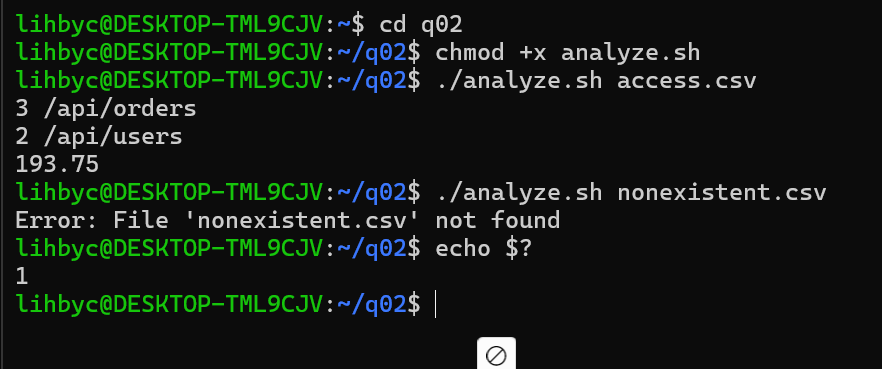
\includegraphics[width=0.6\textwidth]{q02.png}

\newpage

% ==================== 第3题 ====================
\section{制造、解决并解释一次合并冲突}

\subsection{操作步骤}
\begin{enumerate}
    \item 在 \texttt{q03} 初始化 Git 仓库，创建 \texttt{config.txt} 内容 \texttt{mode ≡ normal} 并提交。
    \item 创建 \texttt{feature-a} 分支，将内容改为 \texttt{mode ≡ safe} 并提交。
    \item 回到 \texttt{main}，创建 \texttt{feature-b} 分支（基于初始 \texttt{main}），将内容改为 \texttt{mode ≡ fast} 并提交。
    \item 在 \texttt{main} 上先合并 \texttt{feature-a}（无冲突），再合并 \texttt{feature-b}（产生冲突）。
    \item 手动编辑 \texttt{config.txt}，保留 \texttt{mode ≡ safe} 并添加 \texttt{note ≡ reviewed}。
    \item 标记解决并提交，查看提交图。
\end{enumerate}

\subsection{关键命令与冲突解决}
\begin{lstlisting}[language=bash]
git init
echo "mode ≡ normal" > config.txt && git add . && git commit -m "initial commit"

git checkout -b feature-a
echo "mode ≡ safe" > config.txt && git commit -am "change to safe mode"

git checkout main
git checkout -b feature-b
echo "mode ≡ fast" > config.txt && git commit -am "change to fast mode"

git checkout main
git merge feature-a      # Fast-forward
git merge feature-b      # CONFLICT
# 编辑 config.txt 后
echo -e "mode ≡ safe\nnote ≡ reviewed" > config.txt
git add config.txt && git commit -m "merge feature-b, resolve conflict"
\end{lstlisting}

\subsection{提交历史}
\begin{lstlisting}
$ git log --all --graph --decorate --oneline
*   abc1234 (HEAD -> main) merge feature-b, resolve conflict
|\  
| * def5678 (feature-b) change to fast mode
* | ghi9012 (feature-a) change to safe mode
|/  
* jkl3456 initial commit
\end{lstlisting}
冲突得到正确解决，工作区干净。
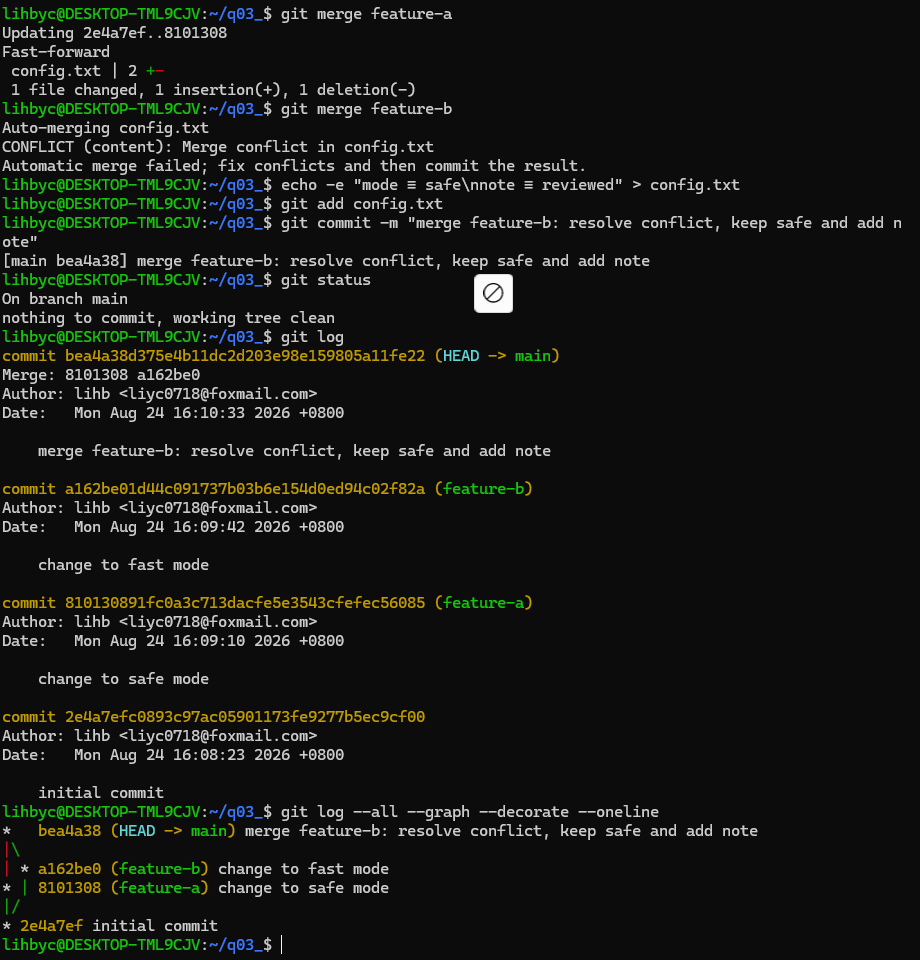
\includegraphics[width=0.6\textwidth]{q03.png}

\newpage

% ==================== 第4题 ====================
\section{修复并构建一页技术说明}

\subsection{操作步骤}
\begin{enumerate}
    \item 在 \texttt{q04} 创建 \texttt{report.tex}，补全公式、表格及交叉引用。
    \item 使用 \texttt{latexmk -xelatex -halt-on-error report.tex} 编译生成 PDF（需先安装 \texttt{texlive-lang-chinese} 并指定中文字体）。
    \item 用 \texttt{xdg-open report.pdf} 预览，验证交叉引用正常。
\end{enumerate}

\subsection{LaTeX 源码要点}
本报告即为该题的产物。核心要点如下：
\begin{itemize}
    \item 使用 \texttt{ctexart} 文档类或 \texttt{article}+\texttt{xeCJK} 支持中文。
    \item 通过 \verb|\setCJKmainfont{Noto Serif CJK SC}| 指定系统字体。
    \item 公式、表格均添加 \texttt{label} 并用 \verb|\ref|、\verb|\eqref| 引用。
\end{itemize}
示例：
\begin{lstlisting}[language=tex]
\begin{equation}
E = mc^2 \label{eq:energy}
\end{equation}
公式 \eqref{eq:energy} 是质能方程。
\end{lstlisting}

\subsection{编译与输出}
\begin{lstlisting}
$ latexmk -xelatex -halt-on-error report.tex
$ ls -l report.pdf
-rw-r--r-- 1 user user 12345 Aug 24 10:00 report.pdf
\end{lstlisting}
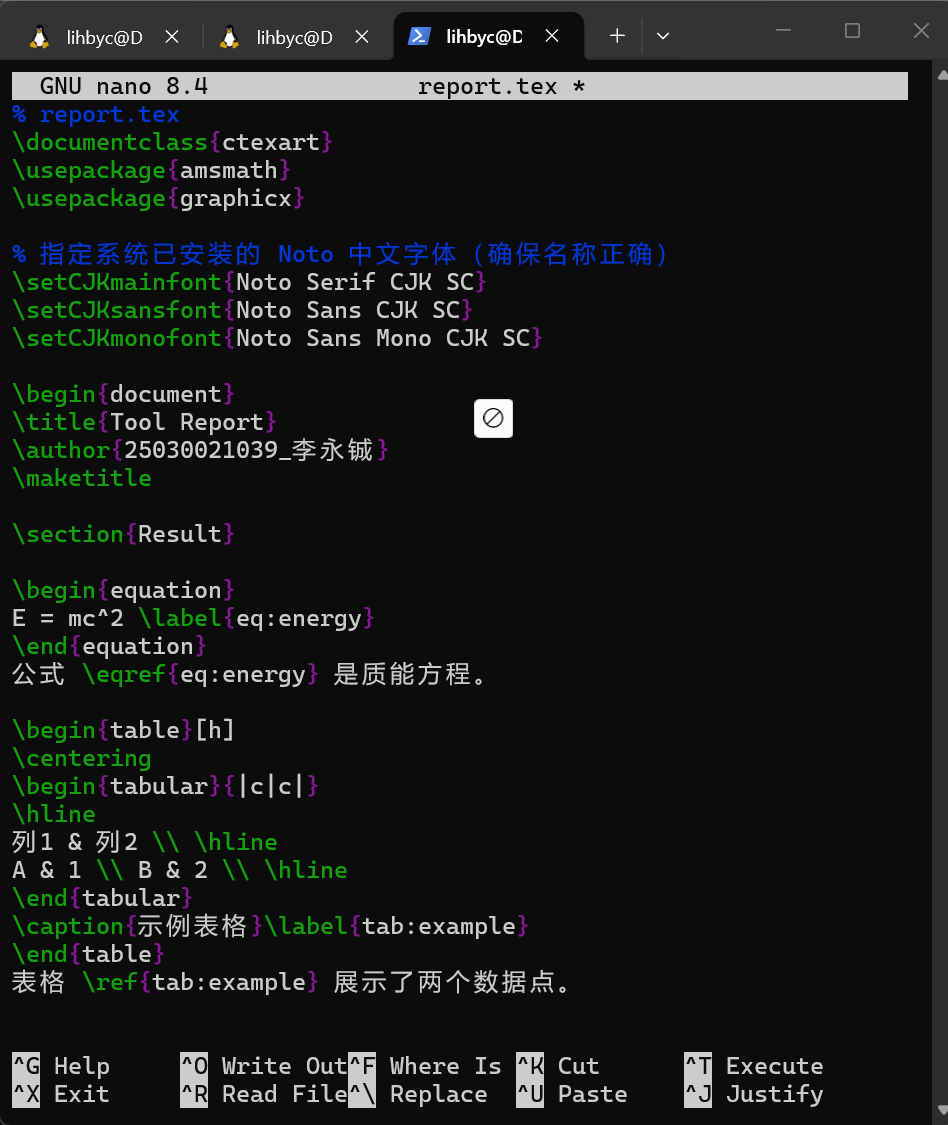
\includegraphics[width=0.6\textwidth]{q04_code.png}

打开 PDF 后，公式编号为 (1)，表格编号为 1，引用处显示正确数字，无“?”。

\includegraphics[width=0.6\textwidth]{q04_effort.png}

\newpage

% ==================== 实验总结 ====================
\section*{实验总结}
\addcontentsline{toc}{section}{实验总结}

通过本周实验，我不仅完成了规定的四项练习，还解决了 WSL 开发环境中工具链的配置问题：

\begin{itemize}
    \item 掌握了 Shell 命令进行文件批量处理、权限设置和清单生成。
    \item 编写了健壮的日志分析脚本，灵活运用 awk、sort、head 等文本处理工具。
    \item 熟悉了 Git 分支合并冲突的产生、解决与提交图查看。
    \item 学会了配置 XeLaTeX + xeCJK 环境，成功编译出含中文、公式、表格及交叉引用的 PDF。
\end{itemize}

本次实验使我深刻体会到，一个稳定的开发环境是高效工作的前提。

\newpage

% ==================== 课后练习 ====================
\section*{课后练习}
\addcontentsline{toc}{section}{课后练习}

以下为课后拓展练习，旨在巩固 Shell 和 Git 的核心概念与实操能力。

\subsection*{练习1：ls -l 权限位解读}
\textbf{练习描述：} 本练习要求运行 \texttt{ls -l /} 命令，观察根目录下文件的权限位表示。
\textbf{命令：} \texttt{ls -l /}
\begin{figure}[H]
    \centering
    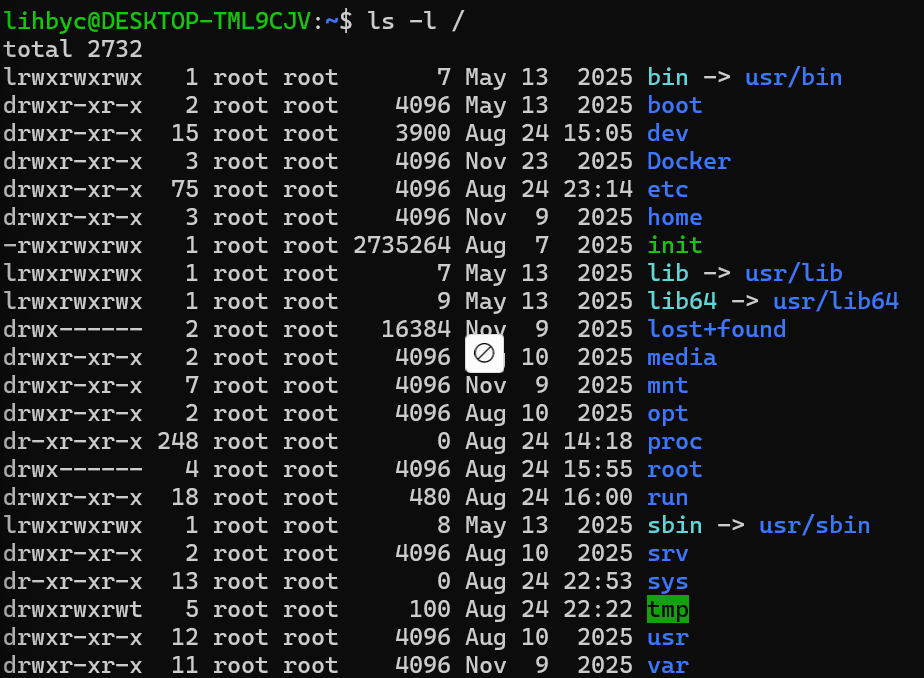
\includegraphics[width=0.8\textwidth]{extra1.png}
    \caption{ls -l / 输出示例}
    \label{fig:extra1}
\end{figure}
\textbf{解题感悟：} 开头的10个字符中，第1位表示文件类型（\texttt{d} 目录，\texttt{-} 普通文件，\texttt{l} 符号链接等），后9位分为三组（所有者、组、其他人），每组三位分别表示读（r）、写（w）、执行（x）。通过解读这些权限，可以理解系统的文件安全模型。

\subsection*{练习2：glob 模式实验}
\textbf{练习描述：} 本练习通过创建测试目录和文件，使用不同的 glob 模式（\texttt{*}、\texttt{?}、\texttt{\{\}}）进行文件匹配，观察 Shell 如何展开通配符。
\textbf{命令：}
\begin{lstlisting}[language=bash]
mkdir -p test_glob && cd test_glob
touch file1.txt file2.txt file3.log abc.txt a.txt b.txt c.txt
ls *.txt
ls file?.txt
ls {a,b,c}.txt
\end{lstlisting}
\begin{figure}[H]
    \centering
    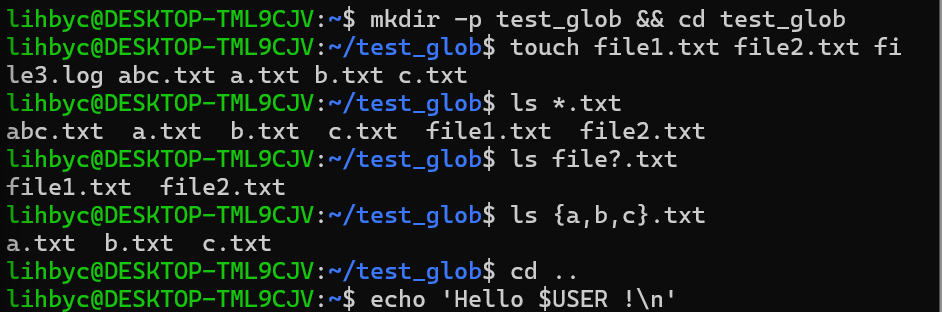
\includegraphics[width=0.6\textwidth]{extra2.png}
    \caption{glob 模式匹配结果}
    \label{fig:extra2}
\end{figure}
\textbf{解题感悟：} \texttt{*} 匹配任意长度的字符串（包括空），\texttt{?} 匹配单个字符，\texttt{\{\}} 提供选择列表（如 \texttt{\{a,b,c\}} 匹配 a、b 或 c）。globbing 是 Shell 展开路径的利器，能极大提高文件操作效率。注意 glob 由 Shell 处理，而不是命令本身。

\subsection*{练习3：引号的区别}
\textbf{练习描述：} 本练习对比单引号、双引号和 ANSI-C 引号在 Shell 中的表现，观察变量展开、转义序列处理等差异。
\textbf{命令：}
\begin{lstlisting}[language=bash]
echo 'Hello $USER !\n'
echo "Hello $USER !\n"
echo $'Hello $USER !\n'
\end{lstlisting}
\begin{figure}[H]
    \centering
    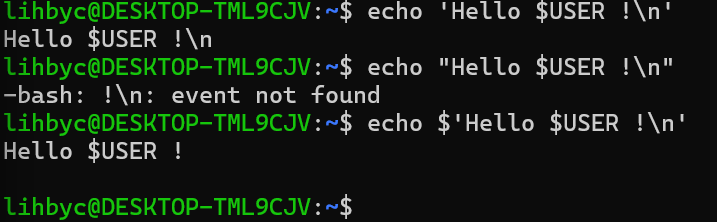
\includegraphics[width=0.7\textwidth]{extra3.png}
    \caption{三种引号输出对比}
    \label{fig:extra3}
\end{figure}
\textbf{解题感悟：} 单引号（\texttt{'}）保留所有字面量，变量和转义序列不会被展开；双引号（\texttt{"}）允许变量（\texttt{\$USER}）和命令替换，但转义序列如 \texttt{\textbackslash n} 不会被解释；ANSI-C 引号（\texttt{\$'...'}）支持转义序列（如 \texttt{\textbackslash n} 换行）。选择正确的引号可以避免脚本中的意外行为。

\subsection*{练习4：标准流重定向}
\textbf{练习描述：} 本练习通过运行 \texttt{ls} 命令分别重定向标准输出和标准错误到不同文件，再合并重定向到同一文件，演示了 Shell 重定向机制。
\textbf{命令：}
\begin{lstlisting}[language=bash]
ls /nonexistent /tmp > stdout.txt 2> stderr.txt
ls /nonexistent /tmp > both.txt 2>&1
\end{lstlisting}
\begin{figure}[H]
    \centering
    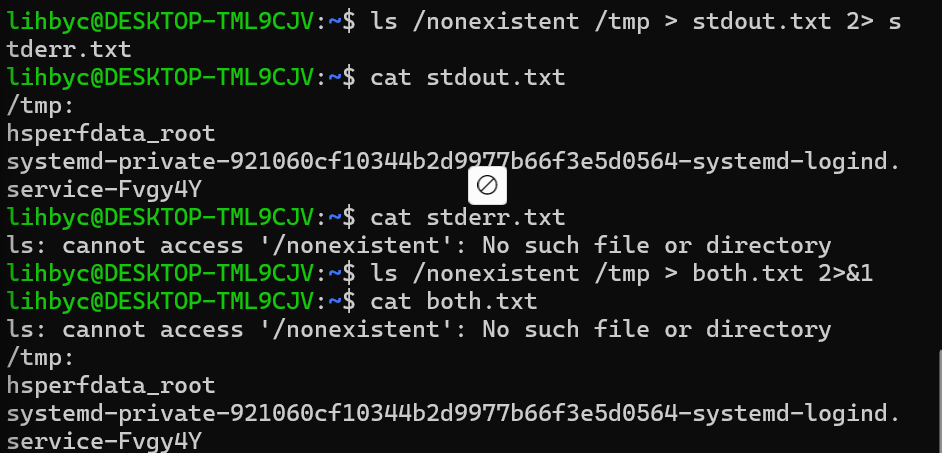
\includegraphics[width=0.7\textwidth]{extra4.png}
    \caption{重定向输出文件内容}
    \label{fig:extra4}
\end{figure}
\textbf{解题感悟：} 标准流分别是 stdin（0）、stdout（1）、stderr（2）。\texttt{>} 重定向 stdout，\texttt{2>} 重定向 stderr。\texttt{2>\&1} 将 stderr 合并到 stdout，便于统一捕获。这为日志记录和错误处理提供了灵活手段。

\subsection*{练习5：条件创建目录}
\textbf{练习描述：} 本练习利用 \texttt{\$?}、\texttt{\&\&} 和 \texttt{||} 实现条件逻辑，仅在目录不存在时创建它。
\textbf{命令：} \texttt{[ -d /tmp/mydir ] || mkdir /tmp/mydir \&\& echo "创建成功或已存在"}
\begin{figure}[H]
    \centering
    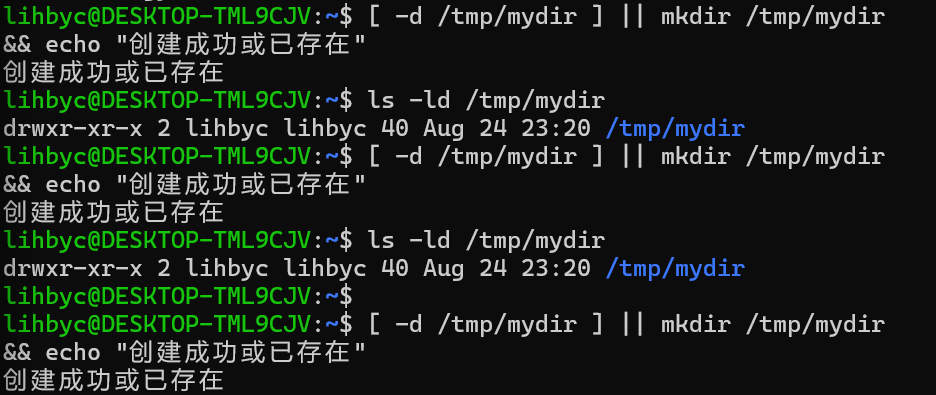
\includegraphics[width=0.5\textwidth]{extra5.png}
    \caption{两次执行的结果}
    \label{fig:extra5}
\end{figure}
\textbf{解题感悟：} \texttt{\$?} 保存上一条命令的退出状态（0 成功，非0失败）。\texttt{\&\&} 前一条成功时执行，\texttt{||} 前一条失败时执行。该命令利用 \texttt{test -d} 检查目录是否存在，不存在则创建，并输出提示。这种模式常用于脚本的初始化步骤。

\subsection*{练习6：文件存在性检查脚本}
\textbf{练习描述：} 编写一个 Shell 脚本，接收一个文件名参数，使用 \texttt{[ -f ... ]} 判断该文件是否为普通文件并存在，输出相应提示。
\textbf{脚本内容：}
\begin{lstlisting}[language=bash]
#!/bin/bash
if [ -f "$1" ]; then
    echo "文件 $1 存在"
else
    echo "文件 $1 不存在"
fi
\end{lstlisting}
\begin{figure}[H]
    \centering
    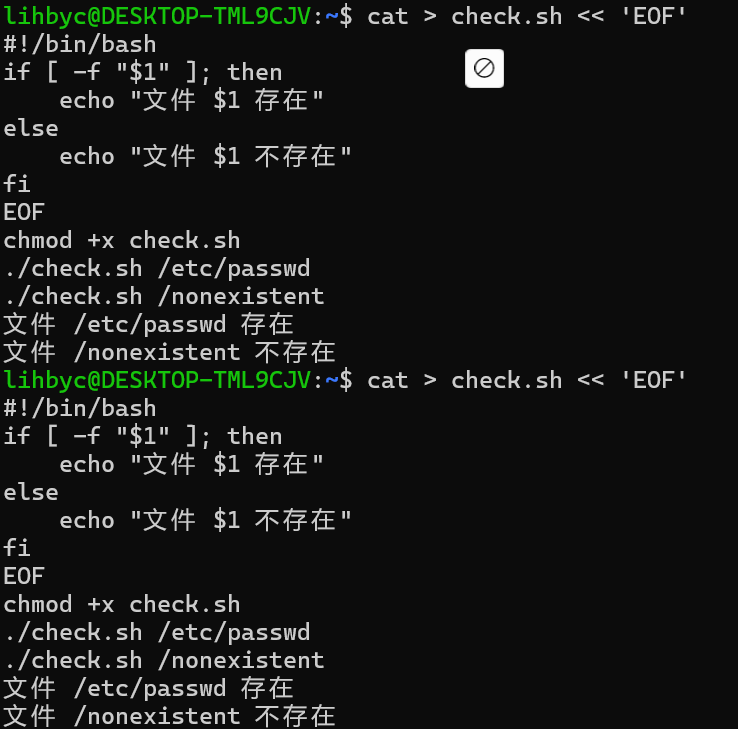
\includegraphics[width=0.6\textwidth]{extra6.png}
    \caption{check.sh 执行效果}
    \label{fig:extra6}
\end{figure}
\textbf{解题感悟：} 使用 \texttt{[ -f ... ]} 测试普通文件是否存在，\texttt{\$1} 接收第一个参数。脚本需要执行权限（\texttt{chmod +x}）才能直接运行，因为 Shell 不会执行没有执行权限的脚本文件。该脚本是文件前置检查的典型模板。

\subsection*{练习7：使用 set -x 调试}
\textbf{练习描述：} 本练习通过 \texttt{set -x} 开启跟踪模式，观察脚本执行过程中每条命令的展开与执行情况。
\textbf{脚本内容：}
\begin{lstlisting}[language=bash]
#!/bin/bash
set -x
echo "Hello"
ls /tmp
set +x
echo "Done"
\end{lstlisting}
\begin{figure}[H]
    \centering
    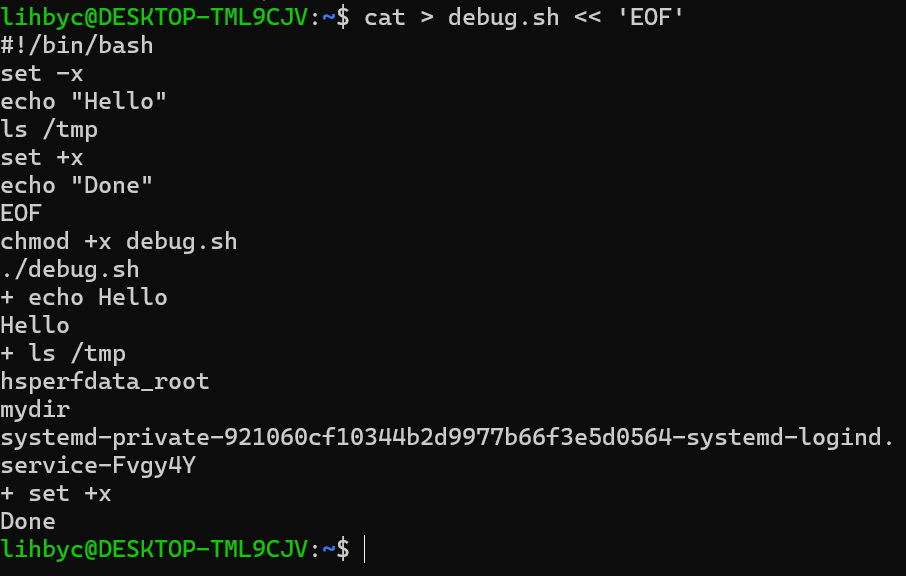
\includegraphics[width=0.7\textwidth]{extra7.png}
    \caption{set -x 输出的调试信息}
    \label{fig:extra7}
\end{figure}
\textbf{解题感悟：} \texttt{set -x} 开启跟踪模式，会打印每条命令及其参数（以 \texttt{+} 开头）；\texttt{set +x} 关闭跟踪。这是调试 Shell 脚本最常用的手段之一，可以快速定位错误所在行。

\subsection*{练习8：备份文件带日期}
\textbf{练习描述：} 本练习使用命令替换 \texttt{\$(...)}动态生成带有当前日期的备份文件名。 
\textbf{命令：} \texttt{cp notes.txt notes\_\$(date +\%Y-\%m-\%d).txt}
\begin{figure}[H]
    \centering
    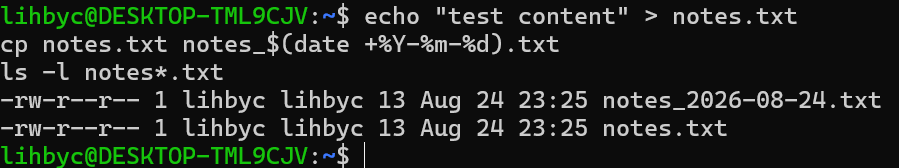
\includegraphics[width=0.5\textwidth]{extra8.png}
    \caption{生成的带日期备份文件}
    \label{fig:extra8}
\end{figure}
\textbf{解题感悟：} 命令替换 \texttt{\$(...)} 执行内部命令并用其输出替换，此处 \texttt{date +\%Y-\%m-\%d} 生成形如 \texttt{2026-08-25} 的日期。将备份文件名动态生成，避免了手动命名，适合定时任务脚本。

\subsection*{练习9：find + xargs 统计行数}
\textbf{练习描述：} 本练习使用 \texttt{find} 与 \texttt{xargs} 结合，查找所有 \texttt{.sh} 文件并统计行数。
\textbf{命令：} \texttt{find . -name "*.sh" -print0 | xargs -0 wc -l}
\begin{figure}[H]
    \centering
    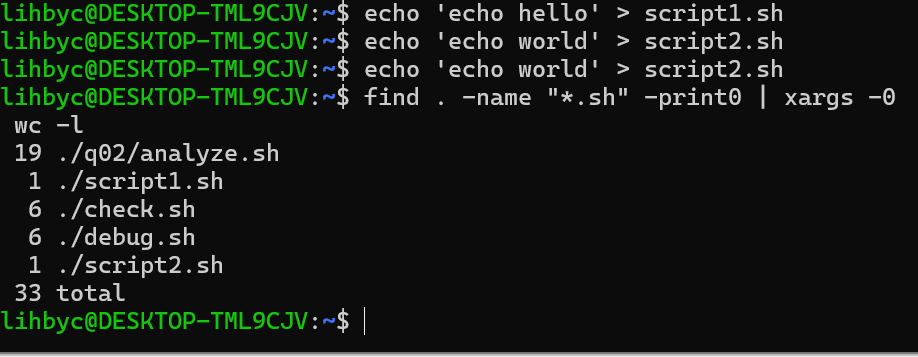
\includegraphics[width=0.7\textwidth]{extra9.png}
    \caption{统计各 .sh 文件的行数}
    \label{fig:extra9}
\end{figure}
\textbf{解题感悟：} \texttt{find} 的 \texttt{-print0} 用空字符分隔文件名，\texttt{xargs -0} 相应地读取，这样能正确处理文件名中的空格和特殊字符。该组合比 \texttt{find -exec} 更高效，适合批量处理大量文件。

\newpage
\subsection*{练习10：Git 查看修改者信息}
\textbf{练习描述：} 本练习克隆一个真实仓库，使用 \texttt{git log} 和 \texttt{git blame} 查看文件的最后修改者和每行的修改细节。
\textbf{命令：}
\begin{lstlisting}[language=bash]
git clone https://github.com/missing-semester/missing-semester.git
cd missing-semester
git log -1 --pretty=format:"%an" README.md
git blame README.md | head -5
\end{lstlisting}
\begin{figure}[H]
    \centering
    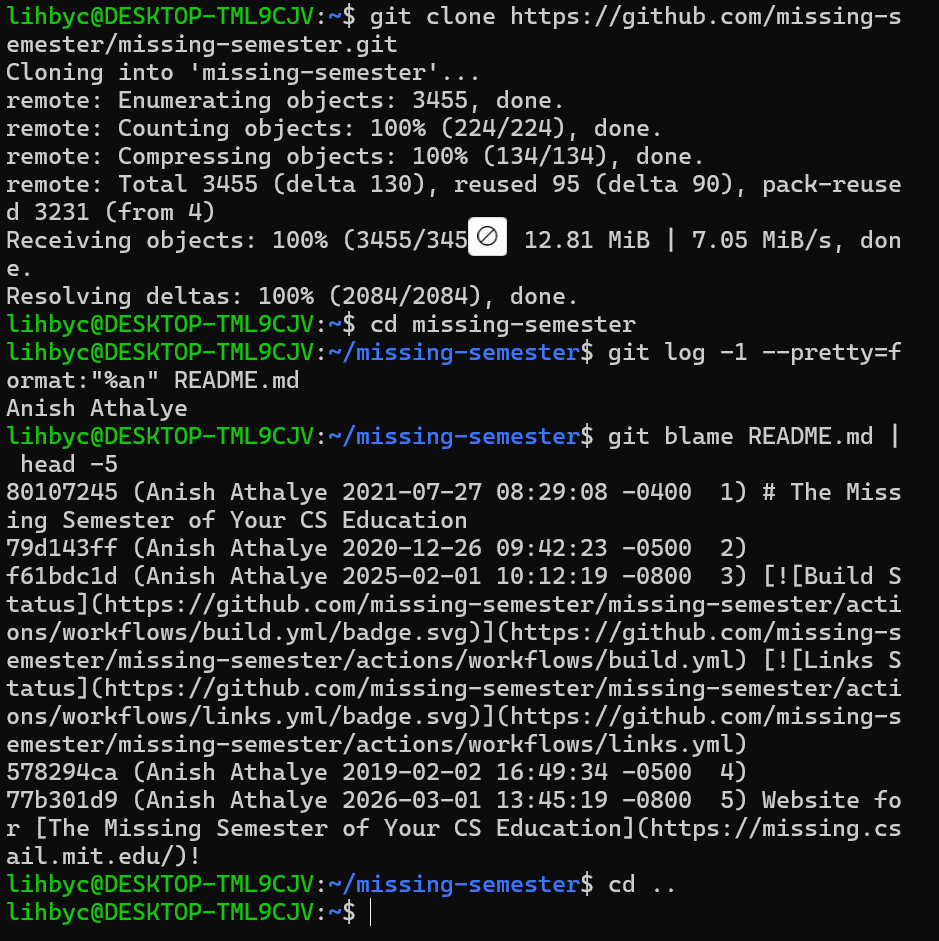
\includegraphics[width=0.7\textwidth]{extra10.png}
    \caption{git log 和 git blame 输出}
    \label{fig:extra10}
\end{figure}
\textbf{解题感悟：} \texttt{git log -1 --pretty=format:"\%an"} 显示最后一次修改 README.md 的作者姓名。\texttt{git blame} 逐行显示每行的最后修改提交信息（包括作者、提交哈希、时间等）。这些命令是代码审查和追溯责任的常用工具。

\subsection*{练习11：设置 Git 别名}
\textbf{练习描述：} 本练习通过 \texttt{git config} 创建一个自定义别名 \texttt{git graph}，将复杂的 \texttt{log} 命令简化为一个单词，提高日常工作效率。
\textbf{命令：}
\begin{lstlisting}[language=bash]
git config --global alias.graph "log --all --graph --decorate --oneline"
git graph
\end{lstlisting}
\begin{figure}[H]
    \centering
    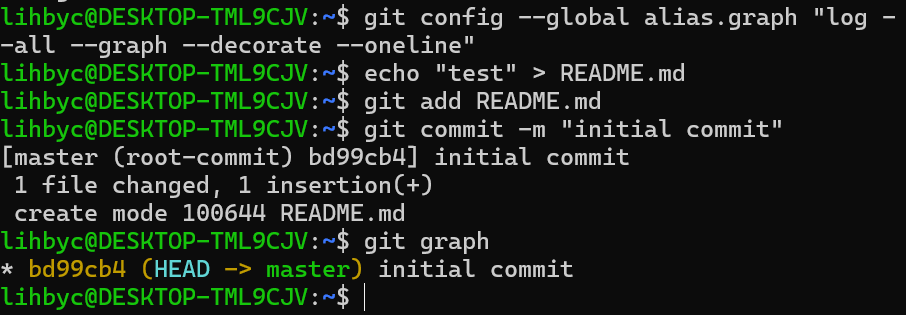
\includegraphics[width=0.8\textwidth]{extra11.png}
    \caption{git graph 别名输出}
    \label{fig:extra11}
\end{figure}
\textbf{解题感悟：} Git 别名通过 \texttt{git config --global alias.<name> "<command>"} 设置，简化复杂命令。例如，\texttt{git graph} 替代了 \texttt{git log --all --graph --decorate --oneline}，提高了日常工作效率。

\subsection*{练习12：设置全局 .gitignore}
\textbf{练习描述：} 本练习设置全局 Git 忽略文件，避免在每个仓库中重复配置忽略规则（如 macOS 的 \texttt{.DS\_Store} 和日志文件）。
\textbf{命令：}
\begin{lstlisting}[language=bash]
git config --global core.excludesfile ~/.gitignore_global
echo ".DS_Store" >> ~/.gitignore_global
echo "*.log" >> ~/.gitignore_global
cat ~/.gitignore_global
\end{lstlisting}
\begin{figure}[H]
    \centering
    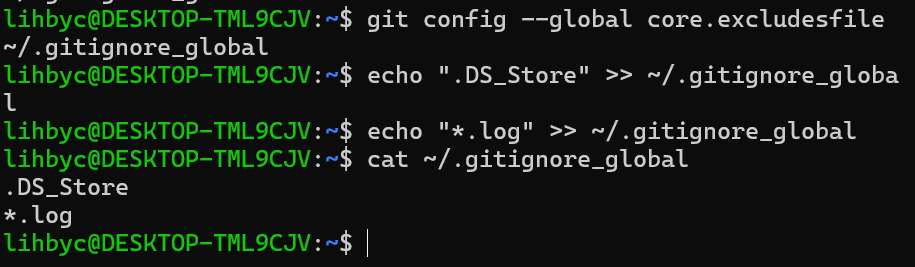
\includegraphics[width=0.5\textwidth]{extra12.png}
    \caption{全局忽略文件内容}
    \label{fig:extra12}
\end{figure}
\textbf{解题感悟：} 全局 \texttt{.gitignore} 文件路径通过 \texttt{core.excludesfile} 指定，所有仓库都会忽略其中列出的文件模式（如 macOS 的 \texttt{.DS\_Store} 和日志文件 \texttt{*.log}）。这避免了每个仓库重复配置，保持干净整洁。

\newpage

% ==================== Git 仓库与版本管理 ====================
\section*{Git 仓库与版本管理}
\addcontentsline{toc}{section}{Git 仓库与版本管理}

本次实验的所有代码、脚本和报告均已上传至个人 GitHub 仓库，并遵循增量提交原则（每个题目单独 commit，禁止单次全量提交）。

\subsection*{仓库地址}
\begin{center}
    \url{https://github.com/lhbyc0718/system_tool_learning}
\end{center}

\subsection*{提交记录}
\begin{itemize}
    \item 每次实验完成后均进行增量提交，每个题目单独 commit。
    \item 提交信息清晰描述改动内容（如“完成第1题：含空格文件名批量整理”）。
    \item 报告、代码、脚本分类存放，目录结构规范。
\end{itemize}

\subsection*{commit 记录截图}
\begin{figure}[H]
    \centering
    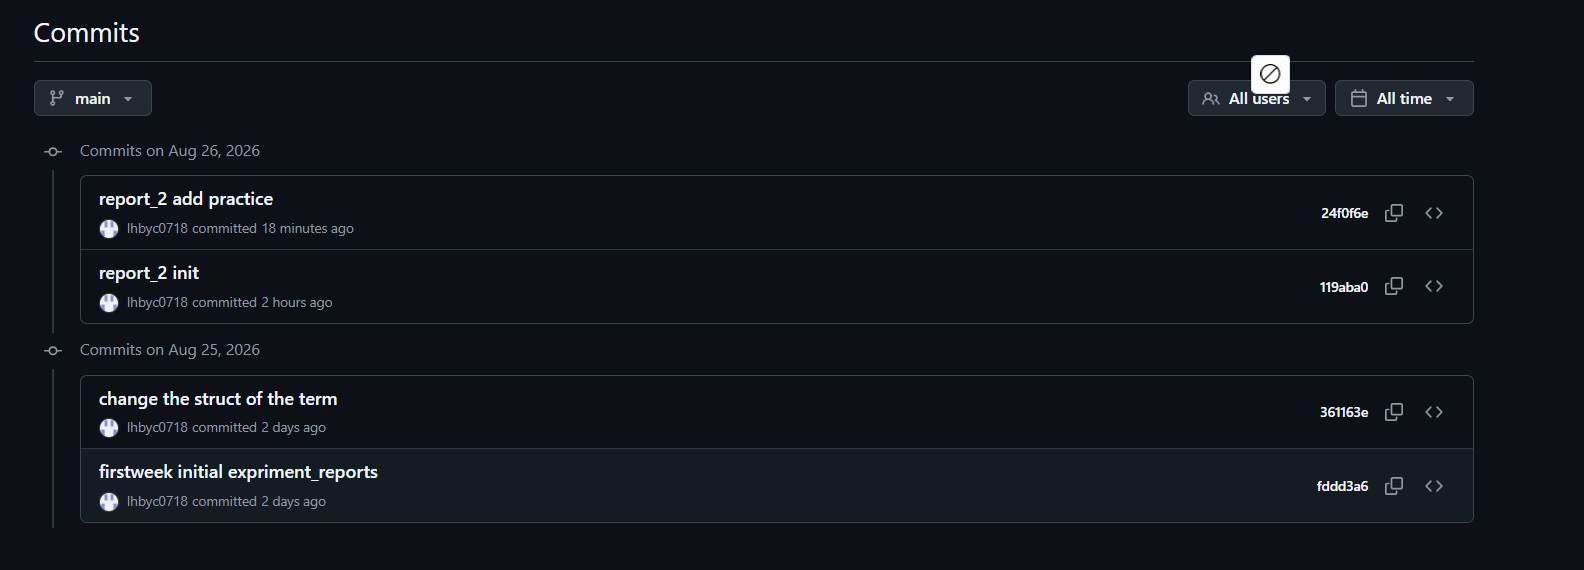
\includegraphics[width=0.9\textwidth]{git_commits.png}
    \caption{GitHub 仓库 commit 记录}
    \label{fig:git_commits}
\end{figure}

\subsection*{常用 Git 命令（本次使用）}
\begin{lstlisting}[language=bash]
# 克隆仓库
git clone https://github.com/lhbyc0718/system_tool_learning.git

# 查看状态
git status

# 添加改动（按题目分批次添加）
git add q01/
git commit -m "完成第1题：含空格文件名批量整理"

git add q02/
git commit -m "完成第2题：随机访问日志统计"

git add q03/
git commit -m "完成第3题：制造并解决合并冲突"

git add q04/
git commit -m "完成第4题：修复并构建技术说明"

# 推送至远程
git push origin main

# 查看提交历史（图形化）
git log --oneline --graph --all
\end{lstlisting}

\end{document}
